\documentclass[a4paper, 10pt, ]{article}

\usepackage[slovak]{babel}

\usepackage[utf8]{inputenc}
\usepackage[T1]{fontenc}

\usepackage[left=4cm,
			right=4cm,
			top=2.1cm,
			bottom=2.6cm,
			footskip=7.5mm,
			twoside,
			marginparwidth=3.5cm,
			%showframe,
			]{geometry}

\usepackage{graphicx}
\usepackage{xcolor}

% ------------------------------

\usepackage{lmodern}

\usepackage[tt={oldstyle=false,proportional=true,monowidth}]{cfr-lm}

% ------------------------------

\usepackage{amsmath}
\usepackage{amssymb}
\usepackage{amsthm}

\usepackage{booktabs}
\usepackage{multirow}
\usepackage{array}
\usepackage{dcolumn}

\usepackage{natbib}

\usepackage[singlelinecheck=true]{subfig}


% ------------------------------


\usepackage{sectsty}
\allsectionsfont{\sffamily}


\usepackage{titlesec}
\titleformat{\paragraph}[hang]{\sffamily  \bfseries}{}{0pt}{}
\titlespacing*{\paragraph}{0mm}{3mm}{1mm}


\usepackage{fancyhdr}
\fancypagestyle{plain}{%
\fancyhf{} % clear all header and footer fields
\fancyfoot[C]{\sffamily {\bfseries \thepage}\ | {\scriptsize\oznacenieCasti}}
\renewcommand{\headrulewidth}{0pt}
\renewcommand{\footrulewidth}{0pt}}
\pagestyle{plain}


% ------------------------------


\makeatletter

	\def\@seccntformat#1{\protect\makebox[0pt][r]{\csname the#1\endcsname\hspace{5mm}}}

	\def\cleardoublepage{\clearpage\if@twoside \ifodd\c@page\else
	\hbox{}
	\vspace*{\fill}
	\begin{center}
	\phantom{}
	\end{center}
	\vspace{\fill}
	\thispagestyle{empty}
	\newpage
	\if@twocolumn\hbox{}\newpage\fi\fi\fi}

	\newcommand\figcaption{\def\@captype{figure}\caption}
	\newcommand\tabcaption{\def\@captype{table}\caption}

\makeatother


% ------------------------------


\def\naT{\mathsf{T}}

\hyphenpenalty=6000
\tolerance=6000


% ------------------------------


\usepackage[pdfauthor={MT},
			pdftitle={AR},
			pdfsubject={},
			pdfkeywords={},
			linkbordercolor = white,
			%citebordercolor = white,
			breaklinks,
			]{hyperref}


\graphicspath{{fig/}}






\begin{document}



\def\oznacenieCasti{ZS2017-AR08}


\fontsize{12pt}{22pt}\selectfont

\centerline{\textsf{Adaptívne riadenie} \hfill \textsf{\oznacenieCasti}}


\fontsize{18pt}{22pt}\selectfont

\begin{flushleft}
	\textbf{\textsf{MRAC vstupno-výstupný}}
\end{flushleft}




\normalsize

\bigskip

\tableofcontents

\bigskip




\vspace{18pt}

\noindent
V tejto časti odvodíme adaptívny algoritmus riadenia, ktorý sa zaraďuje do triedy priame adaptívne riadenie. Pripomeňme priame adaptívne riadenie:

\noindent
Model sústavy je parametrizovaný pomocou ideálnych parametrov zákona riadenia. Pretože tieto parametre sú neznáme, sú priebežne identifikované - adaptované. Výstupom zákona adaptácie sú priamo parametre zákona riadenia.

\medskip
\noindent
Pri odvodení zákona adaptácie sa v tejto časti bude využívať Ljapunovova priama metóda.







\section{SPR prenosové funkcie, MKY lemma}





\subsection{Striktne pozitívne reálne prenosové funkcie}


Pojem \emph{Pozitívne reálna} (PR) a \emph{Striktne pozitívne reálna} (SPR) prenosová funkcia zohráva dôležitú úlohu v analýze stability nie len adaptívnych systémov \cite{IF06}. Je preto dôležité disponovať kritériom, ktoré umožní zistiť, či príslušná prenosová funkcia je SPR (\cite{MH93} str. 164).

Podľa definície 3.5.1 a 3.5.2 v \cite{IF06}, str. 127, prenosová fukcia $G(s)$ komplexnej premennej $s$ sa nazýva pozitívne reálna (PR) ak
\begin{enumerate}
	\item $G(s)$ je reálna pre reálne $s$.
	\item $\Re \left\{ G(s) \right\} \geq 0$ pre všetky $\Re \left\{ s \right\} > 0$.
\end{enumerate}
Prenosová funkcia $G(s)$ je striktne pozitívne reálna (SPR) ak existuje reálne kladné číslo $\varepsilon$ také, že $G(s - \varepsilon)$ je PR.

Prakticky nie je jednoduché zistiť, či uvedené podmienky sú splnené. V~nasledujúcom uvedieme ekvivalentné nutné a~postačujúce podmienky pozitívnej reálnosti. Platnosť týchto podmienok sa dá ľahko overiť.
Prenosová funkcia $G(s)$ je PR keď vyhovuje všetkým nasledujúcim podmienkam
\begin{enumerate}
	\item $G(s)$ je reálna pre všetky reálne~$s$.
	\item Menovateľ $G(s)$ má korene  v~ľavej polrovine komplexnej roviny alebo má reálne korene na imaginárnej osi.
	\item $\Re \left\{ G(j\omega) \right\} \geq 0$ pre všetky reálne $\omega$.
\end{enumerate}

\noindent
Pre vyjadrenie reálnej časti funkcie $G(j\omega)$ je výhodné využiť, že platí:
\begin{equation*}
	\frac{a + jb}{c + jd} = \frac{(a + jb) (c - jd)}{(c + jd) (c - jd)} = \frac{(a + jb) (c - jd)}{c^2 + d^2}
\end{equation*}





\subsection{Meyerova-Kalmanova-Yakubovichova Lemma}
\label{Meyer-Kalman-Yakubovichova Lemma}


Pre danú stabilnú maticu $A$, vektory $b$, $c$ a skalár $d \geq 0$, platí nasledujúce: Ak
\begin{equation*}
	G(s) = d + c^\naT \left( s I - A \right)^{-1} b
\end{equation*}
je SPR, potom pre danú maticu $L = L^\naT > 0$ existujú skalár $v > 0$, vektor $q$ a matica $P =P^\naT > 0$ také, že
\begin{align*}
	A^\naT P + P A &= - q q^\naT - v L \\
	P b	- c	&= \pm q \sqrt{2d}
\end{align*}
Tak znie veta, ktorá, ako sa ukáže, je veľmi užitočná pri návrhu MRAC využívajúceho len vstupno-výstupné informácie.

V tomto kurze ju využijeme v menej všeobecnom tvare: Nech je systém daný trojicou $A_c$, $\overline{B}_c$, $C_c$ a $A_c$ nech je stabilná matica. Ak $ W_m(s) = C_c^\naT \left(  s I - A_c \right)^{-1} \overline{B}_c $ je SPR, potom platí, že
\begin{align*}
	  A_c^\naT P + P A_c &= - Q\\
	  P \overline{B}_c &= C_c
\end{align*}
kde $Q = Q^\naT > 0$. A je to práve fakt, že ak je $W_m(s)$ SPR tak platí $P \overline{B}_c = C_c$, ktorý umožní zredukovať zákon adaptácie tak, že v ňom vystupuje len odchýlka výstupných veličín sústavy a referenčného modelu \cite{Mon74}.










\section{Adaptačná odchýlka}



\subsection{Model sústavy a referenčný model}

Uvažujme sústavu opísanú prenosovou funkciou v tvare
\begin{equation} \label{vvMRAC_PFSustavy}
	\frac{y(s)}{u(s)} = 	k_p 	\frac{Z_p(s)}{R_p(s)}
\end{equation}
kde $Z_p(s)$ je monický Hurwitzov polynóm stupňa $m$, $R_p(s)$ je monický polynóm stupňa $n$ a $k_p$ je tzv. \emph{vysokofrekvenčné zosilnenie sústavy}. \emph{Relatívny stupeň} sústavy je $n^* = n - m$. Predpokladajme, že relatívny stupeň $n^*$ sústavy je známy. Pre zjednodušenie tiež predpokladajme, že aj stupne $n$ a $m$ polynómov sú známe, pričom vo všeobecnosti známe nemusia byť. Koeficienty polynómov $Z_p(s)$ a $R_p(s)$ (parametre sústavy) sú neznáme. Hodnota a znamienko zosilnenia $k_p$ nech je známe.

Sústava v tvare \eqref{vvMRAC_PFSustavy} môže byť reprezentovaná opisom v stavovom priestore v tvare
\begin{subequations}  \label{vvMRACStavOpisSust}
	\begin{align}
		 \dot x  &= A x + b u \\
		 y &= c^\naT x
	\end{align}
\end{subequations}
kde $x$ je vektor stavových veličín sústavy a $A$, $b$, $c^\naT$ sú matice (vektory) zodpovedajúcich rozmerov pričom hodnoty ich prvkov sú neznáme.

Cieľom riadenia je: Nech všetky signály uzavretého regulačného obvodu sú ohraničené a výstupná veličina $y$ sústavy nech sleduje výstupnú veličinu referenčného modelu, ktorý je daný prenosovou funkciou v tvare
\begin{equation} \label{vvMRAC_PFRefModel}
	\frac{y_m(s)}{r(s)} = W_m(s) = k_m \frac{Z_m(s)}{R_m(s)}
\end{equation}
kde $k_m$ je vysokofrekvenčné zosilnenie, $Z_m(s)$ monický Hurwitzov polynóm stupňa $m_m$, $R_m(s)$ monický Hurwitzov polynóm stupňa $n_m$, pričom relatívny stupeň $n^*_m = n_m - m_m = n^*$. Všetky parametre (koeficienty polynómov a $k_m$) referenčného modelu sú známe, dané \uv{projektantom}.










\subsection{Zákon riadenia}

Ako bolo ukázané v predchádzajúcich témach predmetu, zákon riadenia v tvare
\begin{equation} \label{vvMRAC_vseobZakRiaď_i}
	u = {\Theta_1^\star}^\naT \frac{\alpha(s)}{\Lambda(s)} u + {\Theta_2^\star}^\naT \frac{\alpha(s)}{\Lambda(s)} y + \Theta_3^\star y + \Theta_4^\star r
\end{equation}
zabezpečí, že priebeh výstupnej veličiny $y$ sa zhoduje s~priebehom výstupnej veličiny referenčného modelu $y_m$~ak sú parametre zákona vypočítané z podmienok zhody
\begin{subequations}
	\begin{align} \label{vvMRAC_idealTh4}
		\Theta_4^\star &= \frac{k_m}{k_p} \\
		\Lambda &= \Lambda_0 Z_m  \label{vvMRAC_idealLambda} \\
		R_p \left( \Lambda - {\Theta_1^\star}^\naT \alpha(s) \right) -  k_p Z_p 	\left( {\Theta_2^\star}^\naT  \alpha(s) +  \Theta_3^\star\Lambda	 \right) &= Z_p \Lambda_0 R_m
	\end{align}
\end{subequations}

Pretože parametre sústavy \eqref{vvMRAC_PFSustavy} sú neznáme, zákon riadenia \eqref{vvMRAC_vseobZakRiaď_i} nemožno použiť. Použije sa zákon riadenia v tvare
\begin{equation} \label{vvMRAC_vseobZakRiad}
	u = \Theta_1^\naT \frac{\alpha(s)}{\Lambda(s)} u + \Theta_2^\naT \frac{\alpha(s)}{\Lambda(s)} y + \Theta_3 y + \Theta_4 r
\end{equation}
kde $\Theta_1$, $\Theta_2$, $\Theta_3$ a $\Theta_4$ sú odhadmi ideálnych parametrov $\Theta_1^\star$, $\Theta_2^\star$, $\Theta_3^\star$ a $\Theta_4^\star$ v každom čase $t$. Je potrebné nájsť zákon adaptácie, ktorý priebežne generuje (identifikuje) hodnoty $\Theta_1(t)$, $\Theta_2(t)$, $\Theta_3(t)$ a $\Theta_4(t)$.

Pomocné filtre vystupujúce v~zákone riadenia v~stavovom priestore sú (viď predch. článok)
\begin{subequations} \label{vvMRAC_pomFiltre}
	\begin{align}
		\dot \nu_1 &= \Lambda \nu_1 + q u \\
		\dot \nu_2 &= \Lambda \nu_2 + q c^\naT x
	\end{align}
\end{subequations}
a uvažovaný zákon riadenia je
\begin{equation}	\label{vvMRAC_uvZakRiad}
	u = \Theta_c^\naT D X + \Theta_4 r
\end{equation}
kde $ \Theta_c = \begin{bmatrix} \Theta_3^\star  & \Theta_1^\naT & \Theta_2^\naT \end{bmatrix}^\naT$, $\Theta_4$
sú parametre zákona riadenia a
\begin{align*}
	D = \begin{bmatrix}
			c^\naT & 0 & 0 \\
			0 & I & 0 \\
			0 & 0 & I
	\end{bmatrix}
\end{align*}









\subsection{Rovnica adaptačnej odchýlky}



Pridanie pomocných filtrov \eqref{vvMRAC_pomFiltre} k stavovému opisu sústavy \eqref{vvMRACStavOpisSust} vedie k \uv{doplnenej sústave} (viď predch. časti predmetu) v tvare
\begin{subequations} \label{vvMRAC_doplnSustava}
	\begin{align}
		\dot X &=  A_o  X + B_c u \\
		y &= C_c^\naT  X
	\end{align}
\end{subequations}
Parametrizácia doplnenej sústavy \eqref{vvMRAC_doplnSustava} pomocou ideálnych parametrov zákona riadenia sa dosiahne pripočítaním a odpočítaním ideálneho vstupného výrazu $B_c u^\star = B_c {\Theta_c^\star}^\naT D  X + B_c \Theta_4^\star r $
\begin{subequations} \label{vvMRAC_doplnSustava_02}
	\begin{align}
		\dot X &= A_o X + B_c u +  B_c {\Theta_c^\star}^\naT D   X  + B_c  \Theta_4^\star  r - B_c {\Theta_c^\star}^\naT D   X  -  B_c  \Theta_4^\star  r	\\
		\dot X &= \left( A_o + B_c {\Theta_c^\star}^\naT D \right)  X + B_c  \Theta_4^\star r + B_c \left( u - {\Theta_c^\star}^\naT D  X - \Theta_4^\star  r \right)	  \label{vvMRAC_paramDopnSustmedzivyp}
	\end{align}
\end{subequations}
Z predchádzajúcich častí vieme, že $ A_c = A_o + B_c {\Theta_c^\star}^\naT D $, $\overline{B}_c = B_c \Theta_4^\star$ a tiež, že neminimálnu reprezentáciu referenčného modelu \eqref{vvMRAC_PFRefModel} možno (teoreticky) zapísať v~tvare
\begin{subequations} \label{vvMRAC_NeminRefModel}
	\begin{align}
		\dot X_m &= A_c X_m + \overline{B}_c r \\
		y_m &= C_c^\naT X_m
	\end{align}
\end{subequations}
Potom parametrizovaná doplnená sústava \eqref{vvMRAC_paramDopnSustmedzivyp} je
\begin{subequations}
\label{vvMRAC_ParametrizovanaDoplnSustava}
	\begin{align}
		\dot X &= A_c X + \overline{B}_c r + \overline{B}_c \frac{1}{\Theta_4^\star} \left( u - {\Theta_c^\star}^\naT D  X - \Theta_4^\star r \right) \\
		y &= C_c^\naT  X
	\end{align}
\end{subequations}

Definujme \emph{adaptačnú odchýlku} v tvare
\begin{align}
	e &=  X -  X_m \\
	e_1 & = y - y_m
\end{align}
potom:
\begin{subequations} \label{vvMRAC_adaptOdchmedzi}
	\begin{align}
		\dot X - \dot X_m &= A_c \left( X -  X_m \right) + \overline{B}_c r - \overline{B}_c r + \overline{B}_c \frac{1}{\Theta_4^\star} \left( u - {\Theta_c^\star}^\naT D   X - \Theta_4^\star  r \right) \\
		y - y_m &= C_c^\naT \left(  X - X_m \right)
	\end{align}
\end{subequations}
a teda
\begin{subequations}
\label{vvMRAC_adaptOdchSS}
	\begin{align}
		\dot{e} &= A_c e + \overline{B}_c \frac{1}{\Theta_4^\star} \left( u - {\Theta_c^\star}^\naT D   X - \Theta_4^\star r \right) \\
		e_1  &= C_c^\naT e
	\end{align}
\end{subequations}
čo je základná rovnica opisujúca dynamiku adaptačnej odchýlky v stavovom priestore, ktorú možno vyjadriť v~tvare prenosovej funkcie uvážením, že platí
\begin{equation}
	W_m(s) = C_c^\naT \left( s I - A_c \right)^{-1} \overline{B}_c
\end{equation}
Potom \eqref{vvMRAC_adaptOdchSS} v tvare prenosovej funkcie je
\begin{equation} \label{vvMRAC_adaptOdchTF}
	e_1 = W_m(s)  \frac{1}{\Theta_4^\star} \left( u - {\Theta_c^\star}^\naT D  X - \Theta_4^\star r \right)
\end{equation}

Odhadom odchýlky $e_1$ nech je $\hat{e}_1$, ktorá je závislá od odhadov $\Theta_c(t)$, $\Theta_4(t)$.
\begin{equation} \label{vvMRAC_odhadAdaptOdch}
	\hat{e}_1 = W_m(s)  l \left( u - \Theta_c D  X - \Theta_4 r \right)
\end{equation}
kde $l$ je odhadom hodnoty $\frac{1}{\Theta_4^\star}$. Pretože uvažujeme zákon riadenia $ u = \Theta_c^\naT D
 X + \Theta_4 r $, tak $\hat{e}_1 = 0; \quad \forall t$. To znamená, že rovnica \eqref{vvMRAC_odhadAdaptOdch} nie je potrebná pre identifikáciu neznámych parametrov $\Theta_c^\star$, $\Theta_4^\star$ a ako chybu odhadu týchto parametrov možno použiť priamo rovnicu adaptačnej odchýlky \eqref{vvMRAC_adaptOdchTF}.












\section{Zákon adaptácie pri $n^* = 1$}


Uvažujme, že relatívny stupeň sústavy \eqref{vvMRAC_PFSustavy} je $n^* = 1$. Prenosová funkcia referenčného medelu $W_m(s)$ sa volí tak, aby jej relatívny stupeň bol zhodný s relatívnym stupňom sústavy. Relatívny stupeň referenčného modelu $n_m^* = 1$ umožňuje aby prenosová funkcia $W_m(s)$ bola navrhnutá ako striktne pozitívne reálna (SPR).

Nech $W_m(s) = C_c^\naT \left( s I - A_c \right)^{-1} \overline{B}_c$ je SPR. Potom podľa MKY lemmy v časti \ref{Meyer-Kalman-Yakubovichova Lemma} existuje taká matica $P$, pre ktorú platí
\begin{subequations} \label{vvMRAC_dosledkyMKYlemmy}
	\begin{align}
		A_c^\naT P  +  P  A_c  &=  - Q \\
		P  \overline{B}_c &=   C_c
	\end{align}
\end{subequations}
kde $Q = Q^\naT > 0$. Táto skutočnosť sa v ďalšom využije pri voľbe kandidáta na Lyapunovovu funkciu.

Dosadením \eqref{vvMRAC_uvZakRiad} za $u$ do \eqref{vvMRAC_adaptOdchTF} máme
\begin{equation} \label{vvMRAC_adaptOdchmedziDefTF}
	e_1 = W_m(s) \frac{1}{\Theta_4^\star} \left( \theta_c^\naT D X + \theta_4 r \right)
\end{equation}
kde $\theta_c = \Theta_c - \Theta_c^\star$ a $\theta_4 = \Theta_4 - \Theta_4^\star$. Zavedením vektora chyby nastavenia parametrov zákona riadenia $\theta = \begin{bmatrix}  \theta_c^\naT & \theta_4 \end{bmatrix}^\naT$ a signálneho vektora $\omega = \begin{bmatrix} (D X)^\naT & r \end{bmatrix}^\naT$ máme známy tvar adaptačnej odchýlky
\begin{equation} \label{vvMRAC_adaptOdchDefTF}
	e_1 = W_m(s)  \frac{1}{\Theta_4^\star} \left( \theta^\naT \omega \right)
\end{equation}
alebo
\begin{subequations} \label{vvMRAC_adaptOdchDefSS}
	\begin{align}
		\dot{e} &= A_c e + \overline{B}_c \frac{1}{\Theta_4^\star} \left( \theta^\naT \omega \right) \\
		e_1 &= C_c^\naT e
	\end{align}
\end{subequations}

V tomto prípade rovnica \eqref{vvMRAC_adaptOdchDefTF} alebo \eqref{vvMRAC_adaptOdchDefSS} dáva do vzťahu chybu nastavenia parametrov zákona riadenia $\Theta$ a~adaptačnú odchýlku $e_1$ cez SPR prenosovú funkciu.

Predpokladajme, že štruktúra zákona adaptácie je daná diferenciálnou rovnicou všeobecne zapísanou v~tvare
\begin{equation}
	\dot{\theta} = f(e_1, \omega)
\end{equation}
teda aby zákon adaptácie bol funkciou len výstupnej adaptačnej odchýlky $e_1$ a nie aj jej derivácií $e$, pretože tieto nie sú dostupné, nakoľko nie sú dostupné stavové veličiny sústavy.






\begin{figure}[t]
	\centering

	\makebox[\textwidth][c]{%
	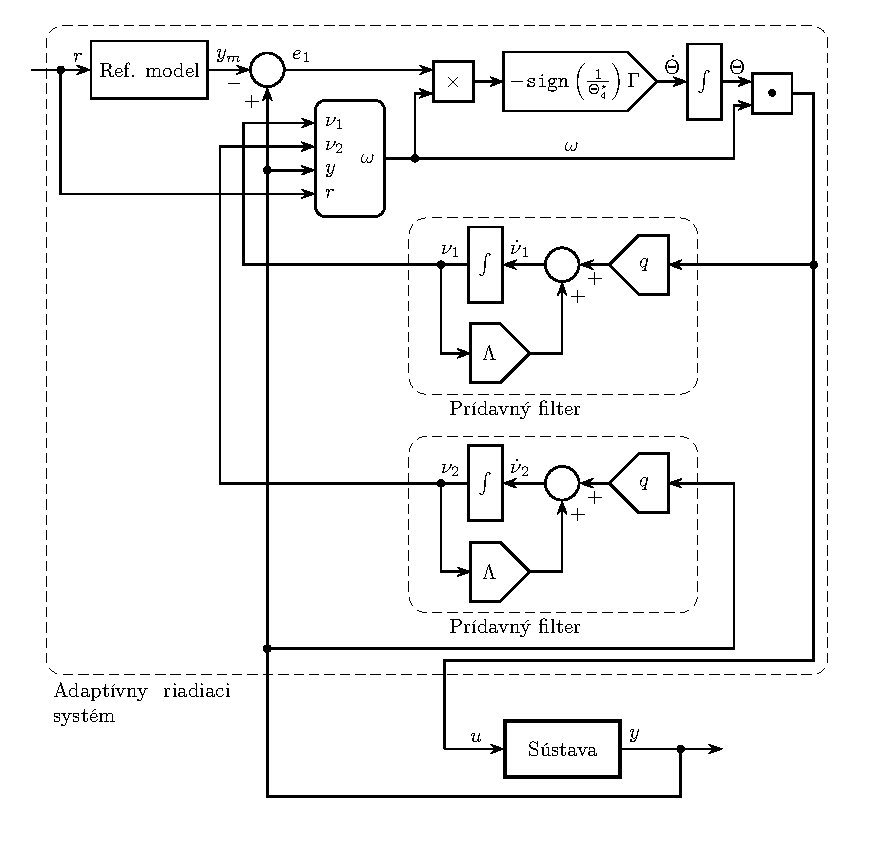
\includegraphics{Obr_vvARS_standalone.pdf}
	}

	\caption{Bloková schéma MRAC so vstupno-výstupnou štruktúrou riadenia pri $n^\star = 1$}
	\label{Bloková schéma MRAC so vstupno-výstupnou štruktúrou riadenia}
\end{figure}




Zvoľme kandidáta na Ljapunovovu funkciu v tvare
\begin{equation}
	V = e^\naT P e + \left| \frac{1}{\Theta_4^\star} \right| \theta^\naT \Gamma^{-1} \theta
\end{equation}
kde $\Gamma > 0$ je ľubovolná diagonálna matica, $\left| \frac{1}{\Theta_4^\star} \right|$ je absolútna hodnota prevrátenej hodnoty parametra $\Theta_4^\star$ a~$P = P^\naT>0$ spĺňa rovnice \eqref{vvMRAC_dosledkyMKYlemmy}, ktoré vyplývajú z~MKY lemmy.
\begin{equation}
	\dot{V} = \dot{e}^\naT P e + e^\naT P \dot{e} + \left| \frac{1}{\Theta_4^\star} \right| \left( \dot{\theta}^\naT \Gamma^{-1} \theta + \theta^\naT \Gamma^{-1} \dot{\theta} \right)
\end{equation}
Poznáme \eqref{vvMRAC_adaptOdchDefSS} odkiaľ $ \dot{e}^\naT = e^\naT A_c^\naT + \omega^\naT \theta \frac{1}{\Theta_4^\star} \overline{B}_c^\naT $, po dosadení týchto výrazov:
\begin{align}
	\dot{V} &= \left( e^\naT A_c^\naT + \omega^\naT \theta \frac{1}{\Theta_4^\star} \overline{B}_c^\naT \right) P e  + e^\naT P \left( A_c  e + \overline{B}_c \frac{1}{\Theta_4^\star} \theta^\naT \omega \right) +  2 \left| \frac{1}{\Theta_4^\star} \right| \theta^\naT \Gamma^{-1} \dot{\theta} \\
	\dot{V} &= e^\naT \left( - Q \right) e + 2 e^\naT P \overline{B}_c \frac{1}{\Theta_4^\star} \theta^\naT \omega + 2 \left| \frac{1}{\Theta_4^\star} \right| \theta^\naT \Gamma^{-1} \dot{\theta}
\end{align}
Pripomeňme, že platí $P \overline{B}_c = {C_c}$ (to vďaka tomu, že $W_m(s)$ je SPR), potom
\begin{align}
	\dot{V} &= e^\naT \left( - Q \right) e + 2 e^\naT C_c \frac{1}{\Theta_4^\star} \theta^\naT \omega + 2 \left| \frac{1}{\Theta_4^\star} \right| \theta^\naT \Gamma^{-1} \dot{\theta}
\end{align}
Všimnime si, že $e^\naT C_c = C_c^\naT e = e_1$. Práve tento moment umožní aby zákon adaptácie $\dot{\theta} = f(e_1, \omega)$ bol funkciou $e_1$ a nie $e$. Časová derivácia $\dot{V}$
\begin{align}
	\dot{V} &= e^\naT \left( - Q \right) e + 2 e_1 \frac{1}{\Theta_4^\star} \theta^\naT \omega + 2 \left| \frac{1}{\Theta_4^\star} \right| \theta^\naT \Gamma^{-1} \dot{\theta}
\end{align}
bude záporne definitná ak
\begin{subequations}
	\begin{align}
	0 &= 2 e_1 \frac{1}{\Theta_4^\star} \theta^\naT \omega + 2 \left| \frac{1}{\Theta_4^\star} \right| \theta^\naT \Gamma^{-1} \dot{\theta} \\
	2 \left| \frac{1}{\Theta_4^\star} \right| \theta^\naT G^{-1} \dot{\theta} &= - 2 e_1 \frac{1}{\Theta_4^\star} \Theta^\naT \omega \\
	\left| \frac{1}{\Theta_4^\star} \right| \Gamma^{-1} \dot{\theta} &= - e_1 \, \texttt{sign}\left(\frac{1}{\Theta_4^\star}\right) \left| \frac{1}{\Theta_4^\star} \right| \omega \\
	\Gamma^{-1} \dot{\theta} &= - \texttt{sign}\left(\frac{1}{\Theta_4^\star}\right) e_1 \omega \\
	\dot{\theta} &= - \texttt{sign}\left(\frac{1}{\Theta_4^\star}\right) e_1 \Gamma \omega
	\end{align}
\end{subequations}
Rovnako ako sme zaviedli vektor $\Theta$, zavedieme aj vektor parametrov zákona riadenia v tvare \\ $\Theta = \begin{bmatrix} \Theta_c^\naT & \Theta_4 \end{bmatrix}^\naT = \begin{bmatrix} {\Theta}_3 & \Theta_1^\naT & \Theta_2^\naT & \Theta_4 \end{bmatrix}^\naT$ a vektor $\omega$ možno zapísať v tvare $\omega = \begin{bmatrix} y & \nu_1^\naT & \nu_2^\naT & r \end{bmatrix}^\naT$. Potom zákon adaptácie je
\begin{equation}
	\dot{\Theta} = - \texttt{sign}\left(\frac{1}{\Theta_4^\star}\right) \Gamma e_1 \omega
\end{equation}
a uvažovaný zákon riadenia možno zapísať v tvare $u = \Theta^\naT \omega$.











\section{Zákon adaptácie pri $n^* = 2$}




\subsection{Priamočiary postup}


Uvažujme relatívny stupeň sústavy \eqref{vvMRAC_PFSustavy} $n^* = 2$. Prenosová funkcia referenčného medelu $W_m(s)$ sa volí tak, aby jej relatívny stupeň bol zhodný s relatívnym stupňom sústavy, teda $n_m^* = 2$. To ale znamená (bez dôkazu), že prenosová funkcia $W_m(s)$ nie je SPR. Preto nie je možné použiť predchádzajúci postup a je ho potrebné modifikovať.

Rovnica pre adaptačnú odchýlku \eqref{vvMRAC_adaptOdchTF}
\begin{equation} \label{vvMRAC_adaptOdchTFn2}
	e_1 = W_m(s)  \frac{1}{\Theta_4^\star} \left( u - {\Theta_c^\star}^\naT D  X - \Theta_4^\star  r \right)
\end{equation}
je stále platná (pri jej odvodení nehral relatívny stupeň sústavy žiadnu úlohu).

Využime identitu $(s+\rho)(s+\rho)^{-1} = 1$ kde $\rho$ je ľubovolná kladná konštanta a~prepíšme rovnicu \eqref{vvMRAC_adaptOdchTF} do tvaru
\begin{equation}  \label{vvMRAC_adaptOdchI}
	e_1 = W_m(s) (s+\rho)(s+\rho)^{-1} \frac{1}{\Theta_4^\star} \left( u - {\Theta_c^\star}^\naT D X - \Theta_4^\star  r \right)
\end{equation}
čo možno prepísať do tvaru
\begin{equation}  \label{vvMRAC_adaptOdchI_02}
	e_1 = W_m(s) (s+\rho) \frac{1}{\Theta_4^\star} \left( u_f - {\Theta^\star}^\naT \omega_f \right)
\end{equation}
kde sme zaviedli $u_f = (s+\rho)^{-1} u$, $\omega_f = (s+\rho)^{-1} \omega$ a ${\Theta^\star}$ je rovnaký ako $\Theta$ avšak obsahuje ideálne parametre.

Nech prenosová funkcia $W_m(s) (s+\rho)$ je zvolená tak, že je to SPR prenosová funkcia. Potom rovnica
\begin{equation}  \label{vvMRAC_adaptOdchI_03}
	e_1 = W_m(s) (s+\rho) \frac{1}{\Theta_4^\star} \left( {\theta}^\naT \omega_f \right)
\end{equation}
kde $\theta = \Theta - \Theta^\star$ dáva do vzťahu chybu nastavenia parametrov zákona riadenia $\theta$~a~adaptačnú udchýlku $e_1$ cez SPR prenosovú funkciu. Reprezentácia rovnice \eqref{vvMRAC_adaptOdchI_03} v~stavovom priestore je
\begin{subequations} \label{vvMRAC_adaptOdchISS}
	\begin{align}
		\dot{e} &= A_c e + \overline{B}_c (s+\rho) \frac{1}{\Theta_4^\star} \theta^\naT \omega_f \\
		e_1 &= C_c^\naT e
	\end{align}
\end{subequations}
kde $s$ teraz predstavuje operátor derivácie $\frac{\text{d}}{\text{d}t}$, rovnako ako bodka \uv{$\,\dot{}\,$} nad $e$. V ďalšom sa tiež stretneme s~takýmto významom symbolu $s$, pričom na to nebudeme zvlášť upozorňovať, konkrétny význam symbolu $s$ vyplynie z kontextu. Preto
\begin{subequations}
	\begin{align}
		se &= A_c e + s \left( \overline{B}_c \frac{1}{\Theta_4^\star} \theta^\naT \omega_f \right) + \rho \left( \overline{B}_c \frac{1}{\Theta_4^\star} \theta^\naT \omega_f \right) \\
		s \left( e - \overline{B}_c \frac{1}{\Theta_4^\star} \theta^\naT \omega_f \right) &= A_c e + \rho \left( \overline{B}_c \frac{1}{\Theta_4^\star} \theta^\naT \omega_f \right)
		\end{align}
\end{subequations}
Označme $e - \overline{B}_c \frac{1}{\Theta_4^\star} \theta^\naT \omega_f = \overline{e} $, potom $e = \overline{B}_c \frac{1}{\Theta_4^\star} \theta^\naT \omega_f + \overline{e} $ a teda
\begin{subequations}
	\begin{align}
		s \overline{e} &= A_c \left( \overline{B}_c \frac{1}{\Theta_4^\star} \theta^\naT \omega_f + \overline{e} \right) + \rho \left( \overline{B}_c \frac{1}{\Theta_4^\star} \theta^\naT \omega_f \right) \\
		e_1 &= C_c^\naT e = C_c^\naT \left( \overline{B}_c \frac{1}{\Theta_4^\star} \theta^\naT \omega_f + \overline{e} \right)
	\end{align}
\end{subequations}
\begin{subequations}
	\begin{align}
		\dot{\overline{e}}
		&=
		A_c
		\overline{e}
		+
		A_c
		\overline{B}_c
		\frac{1}{\Theta_4^\star}
		\theta^\naT
		\omega_f
		+
		\rho
		\overline{B}_c
		\frac{1}{\Theta_4^\star}
		\theta^\naT
		\omega_f
		\\
		e_1
		&=
		C_c^\naT
		\overline{e}
		+
		C_c^\naT
		\overline{B}_c
		\frac{1}{\Theta_4^\star}
		\theta^\naT
		\omega_f
	\end{align}
\end{subequations}
Pretože $C_c^\naT {B}_c = 0$ tak aj $C_c^\naT \overline{B}_c \frac{1}{\Theta_4^\star} \theta^\naT \omega_f = 0 $, potom
\begin{subequations}
	\begin{align}
		\dot{\overline{e}}
		&=
		A_c
		\overline{e}
		+
		\left(
			A_c
			\overline{B}_c
			+
			\rho
			\overline{B}_c
		\right)
		\frac{1}{\Theta_4^\star}
		\theta^\naT
		\omega_f
		\\
		e_1
		&=
		C_c^\naT
		\overline{e}
	\end{align}
\end{subequations}
Označme $A_c \overline{B}_c + \rho \overline{B}_c = B_1 $, potom
\begin{subequations} \label{vvMRAC_adaptOdchISS2}
	\begin{align}
		\dot{\overline{e}}
		&=
		A_c
		\overline{e}
		+
		B_1
		\frac{1}{\Theta_4^\star}
		\theta^\naT
		\omega_f
		\\
		e_1
		&=
		C_c^\naT
		\overline{e}
	\end{align}
\end{subequations}
je stavová reprezentácia systému \eqref{vvMRAC_adaptOdchI_03} daného prenosovou funkciou $W_m(s)(s + \rho)$, pričom $\overline{e}$ je vektor jeho stavových veličín.

Funkcia $W_m(s)(s + \rho) = C_c^\naT \left( s I - A_c \right)^{-1} B_1$ je SPR. Potom podľa MKY lemmy v~časti \ref{Meyer-Kalman-Yakubovichova Lemma} existuje taká matica $P$, pre ktorú platí
\begin{subequations} \label{vvMRAC_dosledkyMKYlemmyn2}
	\begin{align}
		A_c^\naT P  +  P {A_c} &=  - Q \\
		P  B_1 &= {C_c}
	\end{align}
\end{subequations}
kde $Q = Q^\naT > 0$.

Predpokladajme, že štruktúra zákona adaptácie je daná diferenciálnou rovnicou všeobecne zapísanou v~tvare
\begin{equation}
	\dot\theta = f(e_1, \omega_f)
\end{equation}

Zvoľme kandidáta na Ljapunovovu funkciu v~tvare
\begin{equation}
	V = \overline{e}^\naT P \overline{e} + \left| \frac{1}{\Theta_4^\star} \right| \theta^\naT \Gamma^{-1} \theta
\end{equation}
kde $\Gamma > 0$ je ľubovolná diagonálna matica, $\left| \frac{1}{\Theta_4^\star} \right|$ je absolútna hodnota prevrátenej hodnoty parametra $\Theta_4^\star$ a $P = P^\naT>0$ spĺňa rovnice \eqref{vvMRAC_dosledkyMKYlemmyn2}, ktoré vyplývajú z~MKY lemmy.
\begin{equation}
	\dot{V} = \dot{\overline{e}}^\naT P \overline{e} + \overline{e}^\naT P \dot{\overline{e}} + \left| \frac{1}{\Theta_4^\star} \right| \left( \dot{\theta}^\naT \Gamma^{-1} \theta + \theta^\naT \Gamma^{-1} \dot{\theta} \right)
\end{equation}
Poznáme \eqref{vvMRAC_adaptOdchISS2} odkiaľ $ \dot{\overline{e}}^\naT = \overline{e}^\naT A_c^\naT + \omega_f^\naT \theta \frac{1}{\Theta_4^\star} B_1^\naT $, po dosadení týchto výrazov:
\begin{align}
		\dot{V}
		&=
		\left(
			\overline{e}^\naT
			A_c^\naT
			+
			\omega_f^\naT
			\theta
			\frac{1}{\Theta_4^\star}
			B_1^\naT
		\right)
		P
		\overline{e}
		+
		\overline{e}^\naT
		P
		\left(
			A_c
			\overline{e}
			+
			B_1
			\frac{1}{\Theta_4^\star}
			\theta^\naT
			\omega_f
		\right)
		+
		2
		\left| \frac{1}{\Theta_4^\star} \right|
		\theta^\naT
		\Gamma^{-1}
		\dot\theta
		\\
		\dot{V}
		&=
		\overline{e}^\naT
		\left(
			-
			Q
		\right)
		\overline{e}
		+
		2
		\overline{e}^\naT
		P
		B_1
		\frac{1}{\Theta_4^\star}
		\theta^\naT
		\omega_f
		+
		2
		\left| \frac{1}{\Theta_4^\star} \right|
		\theta^\naT
		\Gamma^{-1}
		\dot\theta
\end{align}
Pripomeňme, že platí $P B_1 = {C_c}$, potom
\begin{align}
		\dot{V}
		&=
		\overline{e}^\naT
		\left(
			-
			Q
		\right)
		\overline{e}
		+
		2
		\overline{e}^\naT
		C_c
		\frac{1}{\Theta_4^\star}
		\theta^\naT
		\omega_f
		+
		2
		\left| \frac{1}{\Theta_4^\star} \right|
		\theta^\naT
		\Gamma^{-1}
		\dot\theta
\end{align}
Všimnime si, že $\overline{e}^\naT C_c = C_c^\naT \overline{e} = e_1$.
Časová derivácia $\dot{V}$
\begin{align}
		\dot{V}
		&=
		\overline{e}^\naT
		\left(
			-
			Q
		\right)
		\overline{e}
		+
		2
		e_1
		\frac{1}{\Theta_4^\star}
		\theta^\naT
		\omega_f
		+
		2
		\left| \frac{1}{\Theta_4^\star} \right|
		\theta^\naT
		\Gamma^{-1}
		\dot\theta
\end{align}
bude záporne definitná ak
\begin{subequations}
\begin{align}
	0
	&=
	2
	e_1
	\frac{1}{\Theta_4^\star}
	\theta^\naT
	\omega_f
	+
	2
	\left| \frac{1}{\Theta_4^\star} \right|
	\theta^\naT
	\Gamma^{-1}
	\dot\theta
	\\
	2
	\left| \frac{1}{\Theta_4^\star} \right|
	\theta^\naT
	\Gamma^{-1}
	\dot\theta
	&=
	-
	2
	e_1
	\frac{1}{\Theta_4^\star}
	\theta^\naT
	\omega_f
	\\
	\left| \frac{1}{\Theta_4^\star} \right|
	\Gamma^{-1}
	\dot\theta
	&=
	-
	e_1
	\, \texttt{sign}\left(\frac{1}{\Theta_4^\star}\right)
	\left| \frac{1}{\Theta_4^\star} \right|
	\omega_f
	\\
	\Gamma^{-1}
	\dot\theta
	&=
	-
	\texttt{sign}\left(\frac{1}{\Theta_4^\star}\right)
	e_1
	\omega_f
	\\
	\dot\theta
	&=
	-
	\texttt{sign}\left(\frac{1}{\Theta_4^\star}\right)
	e_1
	\Gamma
	\omega_f
\end{align}
\end{subequations}
Potom zákon adaptácie je
\begin{equation}
	\dot{\Theta}
	=
	-
	\texttt{sign}\left(\frac{1}{\Theta_4^\star}\right)
	\Gamma
	e_1
	\omega_f
\end{equation}

Signálny vektor $\omega_f$ má zložky $\omega_f = \begin{bmatrix} y_f & {\nu_1}_f^\naT & {\nu_2}_f^\naT & r_f \end{bmatrix}^\naT$. Tieto signály získame jednoducho prechodom pôvodných signálov $y$, $\nu_1^\naT$, $\nu_2^\naT$ a $r$ cez filtre s prenosovou funkciou v tvare $\frac{1}{s+\rho}$.

Vstupom do sústavy je $u$. Pri odvodení zákona adaptácie sme ale uvažovali $u_f = (s + \rho)^{-1} u$ odkiaľ $u = (s + \rho)u_f$. Signál $u_f$ možno zapísať aj v tvare $u_f = \Theta^\naT \omega_f$. Teda $u = (s + \rho) \Theta^\naT \omega_f$, z~čoho vyplýva, že
\begin{equation} \label{odvodeneNaznakom}
	u = \Theta^\naT \omega  +  \dot{\Theta}^\naT \omega_f
\end{equation}
Pre objasnenie \eqref{odvodeneNaznakom} naznačíme, že:
\begin{align*}
	&	(s + \rho) \Theta^\naT \omega_f \\
	&	s \left( \Theta^\naT \omega_f \right) + \rho \Theta^\naT \omega_f \\
	&	s \left( \Theta^\naT \right) \omega_f + \Theta^\naT s \left( \omega_f \right) + \rho \Theta^\naT \omega_f \\
	&	\dot{\Theta}^\naT \omega_f + \Theta^\naT s \left( \frac{1}{(s + \rho)} \omega \right) + \rho \Theta^\naT \frac{1}{(s + \rho)} \omega \\
	&	\dot{\Theta}^\naT \omega_f + \Theta^\naT \frac{s}{(s + \rho)} \omega + \Theta^\naT \frac{\rho}{(s + \rho)} \omega \\
	&	\dot{\Theta}^\naT \omega_f + \Theta^\naT \frac{s + \rho}{(s + \rho)} \omega \\
	&	\dot{\Theta}^\naT \omega_f + \Theta^\naT \omega
\end{align*}









\subsection{Metóda doplnenej odchýlky}



Vo všeobecnosti, zákon riadenia, ktorý rieši MRC problém je $u = \Theta^\naT \omega$. Pri jeho dosadení do všeobecne platnej rovnice adaptačnej odchýlky  \eqref{vvMRAC_adaptOdchTF}  máme rovnicu adaptačnej odchýlky v tvare
\begin{equation} \label{vvMRAC_adaptOdchTF_vseob}
	e_1 = W_m(s) \frac{1}{\Theta_4^\star} \theta^\naT \omega
\end{equation}

V rovnici \eqref{vvMRAC_adaptOdchI} sme použili identitu $(s+\rho)(s+\rho)^{-1} = 1$, čo vo všeobecnosti je $L(s)L(s)^{-1} = 1$.

Rovnicu \eqref{vvMRAC_adaptOdchTF_vseob} sme v predchádzajúcom tvare doplnili do tvaru
\begin{equation} \label{vvMRAC_adaptOdchTF_vseobDopoln}
	e_1 = W_m(s) L(s) L(s)^{-1} \frac{1}{\Theta_4^\star} \theta^\naT \omega
\end{equation}
a z rovnice \eqref{vvMRAC_adaptOdchI_02} vyplíva, že \eqref{vvMRAC_adaptOdchTF_vseobDopoln} možno prepísať do tvaru
\begin{equation} \label{vvMRAC_adaptOdchTF_vseobDopoln02}
	e_1 = W_m(s) L(s) \frac{1}{\Theta_4^\star} \theta^\naT L(s)^{-1}  \omega
\end{equation}
Rovnica \eqref{vvMRAC_adaptOdchTF_vseobDopoln02} može byť zapísaná aj v tvare
\begin{equation} \label{vvMRAC_adaptOdchTF_vseobDopoln03}
	e_1  = W_m(s) \frac{1}{\Theta_4^\star} \left( L(s) \theta L(s)^{-1} \right)^\naT \omega
\end{equation}
kde sme vymenili pozície $\frac{1}{\Theta_4^\star}$ a $L(s)$, čo je možné, pretože $\frac{1}{\Theta_4^\star}$ je len konštanta a nie funkcia času, a táto rovnica dáva do vzťahu chybu nastavenia parametrov zákona riadenia s adaptačnou odchýlkou. V stavovom priestore má rovnica \uv{doplnenej} adaptačnej odchýlky \eqref{vvMRAC_adaptOdchTF_vseobDopoln03} tvar
\begin{subequations} \label{vvMRAC_adaptOdchSS_vseobDopoln}
	\begin{align}
		\dot{e} &= A_c e + \overline{B}_c \frac{1}{\Theta_4^\star} \left( L(s) \theta L(s)^{-1} \right)^\naT \omega \\
		e_1 &= C_c^\naT e
	\end{align}
\end{subequations}

Adaptačná odchýlka je definovaná ako $e = X - X_m$ a $e_1 = y - y_m$. Sú dve možnosti ako dosiahnúť aby výsledok odčítania rovníc parametrizovanej doplnenej sústavy, kde stavový vektor je $X$, a neminimálnej reprezentácie referenčného modelu, kde stavový vektor je $X_m$, bol v tvare doplnenej adaptačnej odchýlky \eqref{vvMRAC_adaptOdchSS_vseobDopoln}.






\subsubsection{Prvá možnosť}

Výsledok je rovnaký ako v~predchádzajúcej časti:

Rovnicu parametrizovanej doplnenej sústavy \eqref{vvMRAC_ParametrizovanaDoplnSustava} po dosadení za $u = \Theta^\naT \omega$ možno zapísať v tvare
\begin{subequations} \label{vvMRAC_ParametrizovanaDoplnSustava_vseob}
	\begin{align}
		\dot{X} &= A_c X + \overline{B}_c r + \overline{B}_c \frac{1}{\Theta_4^\star} \theta^\naT \omega \\
		y &= C_c^\naT X
	\end{align}
\end{subequations}

Zavedieme také pravidlo, že keď $W_m(s)$ nie je možné navrhnúť ako SPR, tak v rovnici \eqref{vvMRAC_ParametrizovanaDoplnSustava_vseob} nahradíme $\Theta^\naT$ výrazom $\left( L(s) \theta L(s)^{-1} \right)^\naT$, kde $L(s)$  je dané tým, že $W_m(s)L(s)$ je zvolená ako SPR prenosová funkcia. Teda
\begin{subequations} \label{vvMRAC_ParametrizovanaDoplnSustava_vseobPrav}
	\begin{align}
		\dot{X} &= A_c X + \overline{B}_c r + \overline{B}_c \frac{1}{\Theta_4^\star} \left(  L(s)  \theta  L(s)^{-1}  \right)^\naT \omega \\
		y  &= C_c^\naT X
	\end{align}
\end{subequations}
Pripomeňme
\begin{subequations} \label{vvMRAC_NeminRefModelPrip}
	\begin{align}
		\dot{X}_m &= A_c X_m + \overline{B}_c r \\
		y_m &= C_c^\naT X_m
	\end{align}
\end{subequations}
Odčítaním \eqref{vvMRAC_NeminRefModelPrip} od \eqref{vvMRAC_ParametrizovanaDoplnSustava_vseobPrav} získame rovnicu \uv{doplnenej} adaptačnej odchýlky \eqref{vvMRAC_adaptOdchSS_vseobDopoln}, ktorá zabezpečuje (podrobne ukázané v predchádzajúcom), že chyba nastavenia parametrov zákona riadenia $\theta$ je vo vzťahu z adaptačnou odchýlkou $e_1$ cez SPR prenosovú funkciu.

Pretože rovnica parametrizovanej doplnenej sústavy je modifikovaná podľa zavedeného pravidla, tak aj zákon riadenia je modifikovaný do tvaru $u = \left( L(s) \Theta L(s)^{-1} \right)^\naT \omega$. V prípade, že $L(s) = (s + \rho)$ (ako v predchádzajúcom), tak výraz $L(s) \Theta^\naT L(s)^{-1}$ je funkčne ekvivalentný výrazu
\begin{equation}
	L(s) \Theta^\naT L(s)^{-1} = \Theta^\naT + \dot{\Theta}^\naT L(s)^{-1}
\end{equation}
a teda modifikovaný zákon riadenia má v tomto prípade tvar $u = \Theta^\naT \omega +  \dot{\Theta}^\naT \omega_f$.




\subsubsection{Druhá možnosť}

Výsledkom je algoritmus nazývaný \emph{metóda doplnenej odchýlky}:

Namiesto nahradenia $\theta^\naT$ výrazom $\left( L \theta L^{-1} \right)^\naT$ v rovnici parametrizovanej doplnenej sústavy pridáme vstupný signál v tvare $\frac{1}{\theta_4^\star} \left( \theta - L \theta L^{-1} \right)^\naT \omega$ do referenčného modelu nasledovne
\begin{subequations} \label{vvMRAC_NeminRefModelPrid}
	\begin{align}
		\dot{X}_m
		&=
		A_c
		X_m
		+
		\overline{B}_c
		\left(
			r
			+
			\frac{1}{\Theta_4^\star}
			\left(
			\theta
			-
			L
			\theta
			L^{-1}
			\right)^\naT
			\omega
		\right)
		\\
		y_m
		&=
		C_c^\naT
		X_m
	\end{align}
\end{subequations}
\begin{subequations} \label{vvMRAC_NeminRefModelPrid02}
	\begin{align}
		\dot{X}_m
		&=
		A_c
		X_m
		+
		\overline{B}_c
			r
			+
			\overline{B}_c
			\frac{1}{\Theta_4^\star}
			\left(
				\theta
				-
				L
				\theta
				L^{-1}
			\right)^\naT
		\omega
		\\
		y_m
		&=
		C_c^\naT
		X_m
	\end{align}
\end{subequations}



Rovnica parametrizovanej doplnenej sústavy sa teraz nemení (nemodifikuje)
\begin{subequations} \label{vvMRAC_ParametrizovanaDoplnSustava_vseob02}
	\begin{align}
		\dot{X}
		&=
		A_c
		X
		+
		\overline{B}_c
		r
		+
		\overline{B}_c
		\frac{1}{\Theta_4^\star}
		\theta^\naT
		\omega
\\
		y
		&=
		C_c^\naT
		X
	\end{align}
\end{subequations}
Odčítaním \eqref{vvMRAC_NeminRefModelPrid02} od \eqref{vvMRAC_ParametrizovanaDoplnSustava_vseob02} podľa definície adaptačnej odchýlky máme
\begin{subequations} \label{vvMRAC_adaptOdchSS_MDO01}
	\begin{align}
		\dot{e}
		&=
		A_c
		e
		+
		\overline{B}_c
		\frac{1}{\Theta_4^\star}
		\theta^\naT
		\omega
		-
		\overline{B}_c
		\frac{1}{\Theta_4^\star}
			\left(
				\theta
				-
				L
				\theta
				L^{-1}
			\right)^\naT
		\omega
\\
		e_1
		&=
		C_c^\naT
		e
	\end{align}
\end{subequations}
Výraz
\begin{equation}
	\left(
	\theta
	-
	L
	\theta
	L^{-1}
	\right)
	=
	L
	\left(
	L^{-1}
	\theta
	-
	\theta
	L^{-1}
	\right)
\end{equation}\
Potom
\begin{subequations} \label{vvMRAC_adaptOdchSS_MDO02}
	\begin{align}
		\dot{e}
		&=
		A_c
		e
		+
		\overline{B}_c
		\frac{1}{\Theta_4^\star}
		\theta^\naT
		\omega
		-
		\overline{B}_c
		\frac{1}{\Theta_4^\star}
			\left(
				L
				\left(
					L^{-1}
					\theta
					-
					\theta
					L^{-1}
				\right)
			\right)^\naT
		\omega
		\\
		e_1
		&=
		C_c^\naT
		e
	\end{align}
\end{subequations}
\begin{subequations} \label{vvMRAC_adaptOdchSS_MDO03}
	\begin{align}
		\dot{e}
		&=
		A_c
		e
		+
		\overline{B}_c
		\frac{1}{\Theta_4^\star}
		\theta^\naT
		\omega
		-
		\overline{B}_c
		\frac{1}{\Theta_4^\star}
		L
			\left(
				L^{-1}
				\theta^\naT
				-
				\theta^\naT
				L^{-1}
				\right)
		\omega
		\\
		e_1
		&=
		C_c^\naT
		e
	\end{align}
\end{subequations}

Rovnicu \eqref{vvMRAC_adaptOdchSS_MDO03} je možné prepísať do požadovaného tvaru \eqref{vvMRAC_adaptOdchSS_vseobDopoln} nasledovne:
\begin{subequations} \label{vvMRAC_adaptOdchSS_MDO04}
	\begin{align}
		\dot{e}
		&=
		A_c
		e
		+
		\overline{B}_c
		\frac{1}{\Theta_4^\star}
		\theta^\naT
		\omega
		-
		\overline{B}_c
		\frac{1}{\Theta_4^\star}
		L
		L^{-1}
		\theta^\naT
		\omega
		-
		\overline{B}_c
		\frac{1}{\Theta_4^\star}
		L
		\theta^\naT
		L^{-1}
		\omega
\\
		e_1
		&=
		C_c^\naT
		e
	\end{align}
\end{subequations}
\begin{subequations} \label{vvMRAC_adaptOdchSS_MDO05}
	\begin{align}
		\dot{e}
		&=
		A_c
		e
		+
		\overline{B}_c
		\frac{1}{\Theta_4^\star}
		\theta^\naT
		\omega
		-
		\overline{B}_c
		\frac{1}{\Theta_4^\star}
		\theta^\naT
		\omega
		-
		\overline{B}_c
		\frac{1}{\Theta_4^\star}
		L
		\theta^\naT
		L^{-1}
		\omega
\\
		e_1
		&=
		C_c^\naT
		e
	\end{align}
\end{subequations}
\begin{subequations} \label{vvMRAC_adaptOdchSS_MDO06}
	\begin{align}
		\dot{e}
		&=
		A_c
		e
		+
		\overline{B}_c
		\frac{1}{\Theta_4^\star}
		\left(
			L
			\theta
			L^{-1}
		\right)^\naT
		\omega
\\
		e_1
		&=
		C_c^\naT
		e
	\end{align}
\end{subequations}


Rovnica \eqref{vvMRAC_adaptOdchSS_MDO03} v tvare prenosovej funkcie je
\begin{equation}
	e_1
	=
	W_m
	\frac{1}{\Theta_4^\star}
	\left(
		\theta^\naT
		\omega
		-
		L
			\left(
				L^{-1}
				\theta^\naT
				-
				\theta^\naT
				L^{-1}
				\right)
		\omega
	\right)
\end{equation}
\begin{equation}
	e_1
	=
	W_m
	\frac{1}{\Theta_4^\star}
	\theta^\naT
	\omega
	-
	W_m
	\frac{1}{\Theta_4^\star}
		L
			\left(
				L^{-1}
				\theta^\naT
				-
				\theta^\naT
				L^{-1}
			\right)
		\omega
\end{equation}
Platí
\begin{align}
\begin{split}
	&
	L^{-1}
	\theta^\naT
	-
	\theta^\naT
	L^{-1}
	=
	L^{-1}
	\left(
		\Theta - \Theta^\star
	\right)^\naT
	-
	\left(
		\Theta - \Theta^\star
	\right)^\naT
	L^{-1}
	=\\&=
	\left(
		L^{-1}
		\Theta^\naT
		-
		\Theta^\naT
		L^{-1}
	\right)
	-
	\left(
		L^{-1}
		{\Theta^\star}^\naT
		-
		{\Theta^\star}^\naT
		L^{-1}
	\right)
	=\\&=
	\left(
		L^{-1}
		\Theta^\naT
		-
		\Theta^\naT
		L^{-1}
	\right)
	\end{split}
\end{align}
pretože $\Theta^\star$ nie je funkciou času a teda $L^{-1} {\Theta^\star}^\naT = {\Theta^\star}^\naT  L^{-1}$.
Potom
\begin{equation}
	e_1
	=
	W_m
	\frac{1}{\Theta_4^\star}
	\theta^\naT
	\omega
	-
	W_m
	L
	\frac{1}{\Theta_4^\star}
	\left(
		L^{-1}
		\Theta^\naT
		\omega
		-
		\Theta^\naT
		L^{-1}
		\omega
	\right)
\end{equation}
\begin{equation}
	e_1
	=
	W_m
	\frac{1}{\Theta_4^\star}
	\theta^\naT
	\omega
	-
	W_m
	L
	\frac{1}{\Theta_4^\star}
	\left(
		L^{-1}
		u
		-
		\Theta^\naT
		\omega_f
	\right)
\end{equation}
kde označíme:
$e_m = W_m \frac{1}{\Theta_4^\star} \theta^\naT \omega$ je odchýlka medzi výstupom pôvodného nemodifikovaného referenčného modelu a signál $e_d = W_m L \frac{1}{\Theta_4^\star} \left( L^{-1} u - \Theta^\naT \omega_f \right) $ sa pridá k tejto odchýlke, čím vznikne modifikovaný signál $e_1$~a~tento sa použije v zákone adaptácie.

Rovnicu parametrizovanej doplnenej sústavy \eqref{vvMRAC_ParametrizovanaDoplnSustava_vseob02} sme nezmenili, preto sa v tomto prípade nemení ani zákon riadenia $u = \Theta^\naT \omega$.













\begin{figure}[t]
	\centering

	\makebox[\textwidth][c]{%
	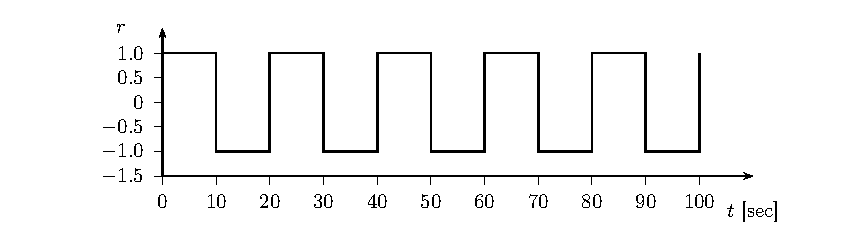
\includegraphics{Obr_cv5Vzor_1.pdf}
	}

	\caption{Referenčný sigál $r$}
	\label{Referenčný sigál $r$ 6cv}

\end{figure}



\begin{figure}[t]
	\centering

	\makebox[\textwidth][c]{%
	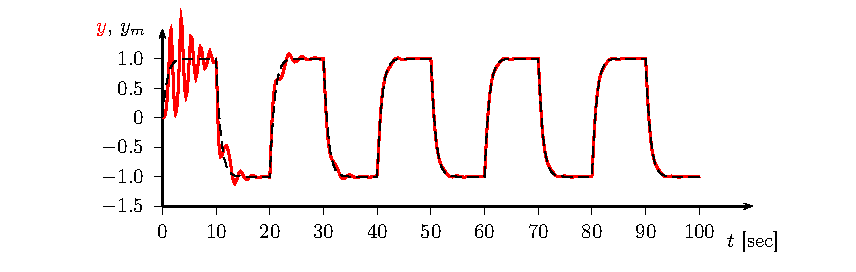
\includegraphics{Obr_cv5Vzor_2.pdf}
	}

	\caption{Výsledok simulácie}
	\label{Výsledok simulácie 6cv}

\end{figure}










\section{Cvičenie ôsme}
\label{cvicosme}



\begin{enumerate}

	\item Uvažujme sústavu danú v dvoch hraničných pracovných bodoch:
	\begin{align}
		G_{OP_1}
		&=
		0,1659 \frac{s + 22}{ s^2 + 3,1423 s + 2,6539}
		\label{plantModel12} \\
		G_{OP_2}
		&=
		0,1669 \frac{s + 20,7618}{s^2 + 2,3422s + 2,7293}
		\label{plantModel22}
	\end{align}
	\begin{itemize}
		\item Určte \emph{nominálnu} prenosovú funkciu sústavy tak, že jej koeficienty sú	priemery hodnôt oboch prenosových funkcií \eqref{plantModel12} a \eqref{plantModel22}.
		\item Pre nominálnu prenosovú funkciu sústavy určte polynómy $Z_p$, $R_p$ a~zosilnenie $k_p$ pričom
		\begin{equation} \label{C_PFsustavy_MRCp2}
			\frac{y(s)}{u(s)}
			=
			k_p
			\frac{Z_p(s)}{R_p(s)}
		\end{equation}
	kde $Z_p(s)$ je monický polynóm stupňa $m$, $R_p(s)$ je monický polynóm stupňa $n$ a $k_p$ je tzv. \emph{vysokofrekvenčné zosilnenie sústavy}. \emph{Relatívny stupeň} sústavy je $n^* = n - m$.
	\end{itemize}


	\item Pre nominálnu prenosovú funkciu sústavy navrhnite adaptívne riadenie s referenčným modelom so vsupno-výstupnou štruktúrou zákona riadenia (merateľný je len výstup sústavy a samozrejme vstup sústavy). Pre odvodenie zákona adaptácie použite priamu Lyapunovou metódu. Nech referenčný model je v tvare
	\begin{equation}
		W_m(s)
		=
		\frac{s + 3}{ s^2 + 3.5 s + 3}
	\end{equation}

	\begin{itemize}
		\item Určte zákon riadenia, ktorý sa bude používať v adaptívnom riadiacom systéme.
		\item Vypočítajte ideálne parametre zákona riadenia.
		\item Zistite, či $W_m(s)$ je striktne pozitívne reálna (SPR) prenosová funkcia.
		\item Napíšte rovnicu výstupnej adaptačnej odchýlky $e_1$.
		\item Pre systém diferenciálnych rovníc ($\dot e$, $\dot \theta$), kde $\dot \theta$ sa najskôr uvažuje vo všeobecnom tvare (na začiatku odvodenia sa uvažuje len všeob. funkcia $f$) zvoľte kandidáta na Lyapunovovu funkciu a odvoďte (skonkretizujte) predpis (pravú stranu) pre $\dot \theta$.
		\item Určte zákon adaptácie, ktorý sa bude používať v adaptívnom riadiacom systéme
		\item Zvoľte $\Gamma$ (jednoducho, zvoľte všetky ľubovolne voliteľné prvky zákona/zákonov adaptácie).
		\item Začiatočné hodnoty adaptovaných parametrov zvoľte nulové.
		\item Zostavte adaptívny riadiaci systém (simulačnú schému) a pridajte ho k~simulovanej sústave.
		\item Použite obdĺžnikový referenčný signál $r$ ako na Obr.~\ref{Referenčný sigál $r$ 6cv}. Vzorové výsledky simulácie sú na Obr.~\ref{Výsledok simulácie 6cv}.
	\end{itemize}

\end{enumerate}















\section{Cvičenie deviate a desiate}
\label{cvic910}


\subsection{Referát MRAC vstupno-výstupný pri ($n^* = 2$)}


\noindent
Riadny termín odovzdania: do(vrátane) \textbf{\color{red}\ldots} %.

\bigskip

\noindent
Odovzdanie po riadnom termíne sa pokutuje odčítaním bodov od výsledného hodnotenia. Za každý začatý deň po riadnom termíne sa odčítajú 3 body.

\noindent
1. deň po riadnom termíne: $H-3$ body,\\
2. deň po riadnom termíne: $H-3$ body,\\
3. deň po riadnom termíne: $H-3$ bodov,\\
4. deň po riadnom termíne: $H-3$ bodov,\\
5. deň po riadnom termíne: $H-3$ bodov,\\
kde $H$ je počet bodov pridelených referátu -- $H$ ako hodnotenie. Päť a viac dní po riadnom termíne už nie je možné referát odovzdať a študent/študentka získa $0$~bodov. Minimálny počet bodov za referát je $0$~bodov. Maximálny počet bodov za referát je $15$ bodov.


\bigskip

\noindent
Pre prácu na zadaní a referáte sú vyhradené cvičenia v~9. a~10. týždni semestra.




\subsection{Zadanie}

\noindent
Navrhnite adaptívny riadiaci systém pre riadenie kurzu nákladnej lode. Riadenou (výstupnou) veličinou je kurz (uhol otočenia) lode, pričom táto veličina je merateľná a akčným zásahom je výchylka (uhol) kormidla. Pri návrhu využite prístup, ktorého základom je Lyapunovova teória stability. Vypracujte referát o~návrhu adaptívneho riadiaceho systému pre riadenie kurzu nákladnej lode.

Pohyb lode opisuje diferenciálna rovnica v tvare \cite{PY98}
\begin{equation} \label{DRlode}
	\dddot{\varphi}(t)
	+
	\left(
		\frac{\tau_1 + \tau_2}{\tau_1 \tau_2}
	\right)
	\ddot{\varphi}(t)
	+
	\left(
		\frac{1}{\tau_1 \tau_2}
	\right)
	\dot{\varphi}(t)
	=
	\frac{K}{\tau_1 \tau_2}
	\left(
		\tau_3
		\dot{\delta}(t)
		+
		\delta(t)
	\right)
\end{equation}
kde $\varphi$ je uhol natočenia lode v radiánoch (azimut, kurz lode), $\delta$ je uhol vychýlenia kormidla v radiánoch. Parametre v rovnici \eqref{DRlode} sú definované nasledovne
\begin{align}
	K &= K_0 \frac{v}{L} \\
	\tau_i &= \tau_{i0} \frac{L}{v} \qquad i=1,2,3
\end{align}
kde $v$ je rýchlosť lode v smere danom uhlom $\varphi$ v metroch za sekundu, $L$ je dĺžka lode v metroch a $K_0$, $\tau_{10}$, $\tau_{20}$, $\tau_{30}$ sú konštanty závislé na veľkom množstve faktorov (typ lode atď.).

Požiadavky na dynamiku kormidlovania nákladnej lode nech sú definované referenčným modelom v tvare prenosovej funkcie:
\begin{equation}
	\frac{y_m(s)}{r(s)}
	=
	\frac{0,0025 }{s^2 + 0,1 s + 0,0025}
\end{equation}
kde $r$ je referenčný kurz a $y_m$ je požadovaná reakcia lode. Cieľom riadenia je zabezpečiť aby sa reakcia lode na referenčný signál zhodovala s reakciou referenčného modelu.

Pri simulačnom overovaní navrhnutého riadiaceho systému použite periodický referenčný signál s amplitúdou $5^\circ$, s periódou z intervalu 500 až 1000 sekúnd a so sínusovým, obdĺžnikovým alebo pílovitým tvarom. Číselné hodnoty parametrov pre simulačný model lode sú:
\begin{align*}
	L &= 161 \\
	K_0 &= -3,86 \\
	\tau_{10} &=  5,66 \\
	\tau_{20} &=  0,38 \\
	\tau_{30} &=  0,89 \\
	v &= 5
\end{align*}





























\section{Otázky a úlohy}


\noindent
Nasledujúce nepatrí k predchádzajúcej časti \emph{\ref{cvic910} Cvičenie deviate a desiate}.



\begin{enumerate}


	\item Zistite či je prenosová funkcia $G(s)$ striktne pozitívne reálna (SPR).
	\begin{equation*}
		G(s) = \frac{2\,s + 1}{ (3\,s + 1) (s + 1)}
	\end{equation*}


	\item Pre aké hodnoty $a$, $b$, $c$ je prenosová funkcia $\displaystyle G(s) = \frac{as + 1}{ \left( bs + 1 \right)   \left( cs + 1 \right)   }$ striktne pozitívne reálna.


	\item Schematicky znázornite MRAC vstupno-výstupný pri $n^\star = 1$

	\item Schematicky znázornite MRAC vstupno-výstupný pri $n^\star = 2$

	\item Čo je cieľom riadenia pri návrhu adaptívneho riadiaceho systému s referenčným modelom so zákonom adaptácie navrhnutým pomocou Lyapunovovej teórie stability?


	\item Je daný model systému
	\begin{align*}
		\dot{x}_1(t) &= x_2(t) \\
		\dot{x}_2(t) &= -a_1 x_2(t) - a_0 x_1(t) + b_0 u(t) \\
		y(t) & = x_1(t)
	\end{align*}
	kde $a_0, a_1, b_0 > 0$ sú neznáme parametre systému, $u(t)$ je vstup, $y(t)$ je výstup a $x_1(t)$, $x_2(t)$ sú stavové veličiny systému. Tiež je daný referenčný model v tvare
	\begin{align*}
		\begin{bmatrix}
			\dot{x}_{1m}(t) \\ \dot{x}_{2m}(t)
		\end{bmatrix}
		&=
		\begin{bmatrix}
			0 & 1 \\ -a_{0m} & -a_{1m}
		\end{bmatrix}
		\begin{bmatrix}
			x_{1m}(t)  \\ x_{2m}(t)
		\end{bmatrix}
		+
		\begin{bmatrix}
			0  \\  b_{0m}
		\end{bmatrix}
		r(t) \\
		y_m(t)
		&=
		\begin{bmatrix}
			1 & 0
		\end{bmatrix}
		\begin{bmatrix}
			x_{1m}(t)  \\ x_{2m}(t)
		\end{bmatrix}
	\end{align*}
	kde $a_{0m}, a_{1m}, b_{0m} > 0$ sú známe parametre referenčného modelu, $r(t)$ je referenčný signál, $y_m(t)$ je výstup a~$x_{1m}(t)$, $x_{2m}(t)$ sú stavové veličiny referenčného modelu.
	\begin{enumerate}
		\item Napíšte model systému v tvare prenosovej funkcie \label{odvodtePrenosFcn}
		\begin{equation*}
			\frac{y(s)}{u(s)}
			=
			k_p
			\frac{Z_p(s)}{R_p(s)}
		\end{equation*}
		kde $Z_p(s)$ je monický, hurwitzov polynóm stupňa $m$, $R_p(s)$ je monický polynóm stupňa $n$ a~$k_p$~je  vysokofrekvenčné zosilnenie sústavy. Napíšte referenčný model v tvare prenosovej funkcie
		\begin{equation*}
			\frac{y_m(s)}{r(s)}
			=
			W_m(s)
			=
			k_m
			\frac{Z_m(s)}{R_m(s)}
		\end{equation*}
		kde $k_m$ je vysokofrekvenčné zosilnenie referenčného modelu, polynóm $Z_m(s)$ je monický Hurwitzov polynóm stupňa $m_m$, $R_m(s)$ monický Hurwitzov polynóm stupňa $n_m$.

		\item Ideálnym cieľom riadenia je $y = y_m$. Navrhnite ideálny zákon riadenia v~tvare
		\begin{equation*}
			u
			=
			{\Theta_1^\star}^\naT
			\frac{\alpha(s)}{\Lambda(s)}
			u
			+
			{\Theta_2^\star}^\naT
			\frac{\alpha(s)}{\Lambda(s)}
			y
			+
			\Theta_3^\star
			y
			+
			\Theta_4^\star
			r
		\end{equation*}
		kde $\alpha(s)$ je vektor obsahujúci mocniny $s$, $\alpha(s) = \begin{bmatrix} s^{n-2}, \ldots,s, 1 \end{bmatrix}^{\mathsf{T}}$ ak $n\geq 2$, inak $\alpha(s) = 0$. Vektory $\Theta_1^\star, \Theta_2^\star \in \mathbb{R}^{n-1}$ a  skaláry $\Theta_3^\star, \Theta_4^\star \in \mathbb{R}^1$ sú konštantné parametre zákona riadenia, ktorých hodnoty hľadáme.  $\Lambda(s)$ je ľubovolný monický Hurwitzov polynóm stupňa $n-1$ obsahujúci $Z_m(s)$ ako faktor
		\begin{equation*}
			\Lambda(s) = \Lambda_0(s) Z_m(s)
		\end{equation*}
		a teda aj $\Lambda_0(s)$ je ľubovolný monický Hurwitzov polynóm zodpovedajúceho stupňa.

		\item Cieľom riadenia je $y \to y_m$ a stabilita celého riadiaceho systému. Navrhnite adaptívny riadiaci systém, pričom uvažujte model riadeného systému v~tvare prenosovej funkcie  a tiež referenčný model v tvare prenosovej funkcie z~predchádzajúceho bodu \ref{odvodtePrenosFcn}.

	\end{enumerate}
\end{enumerate}











\bibliography{misc/Bib_KurzAR}{}
\bibliographystyle{plain}



\end{document}
